\section{Background}\label{sec:background}

\begin{figure*}[t]
    \centering

    % ---------------- Row 1: Old Model ----------------
    \begin{subfigure}[t]{\textwidth}
        \centering
        \begin{minipage}[t]{0.3\textwidth}
            \centering
            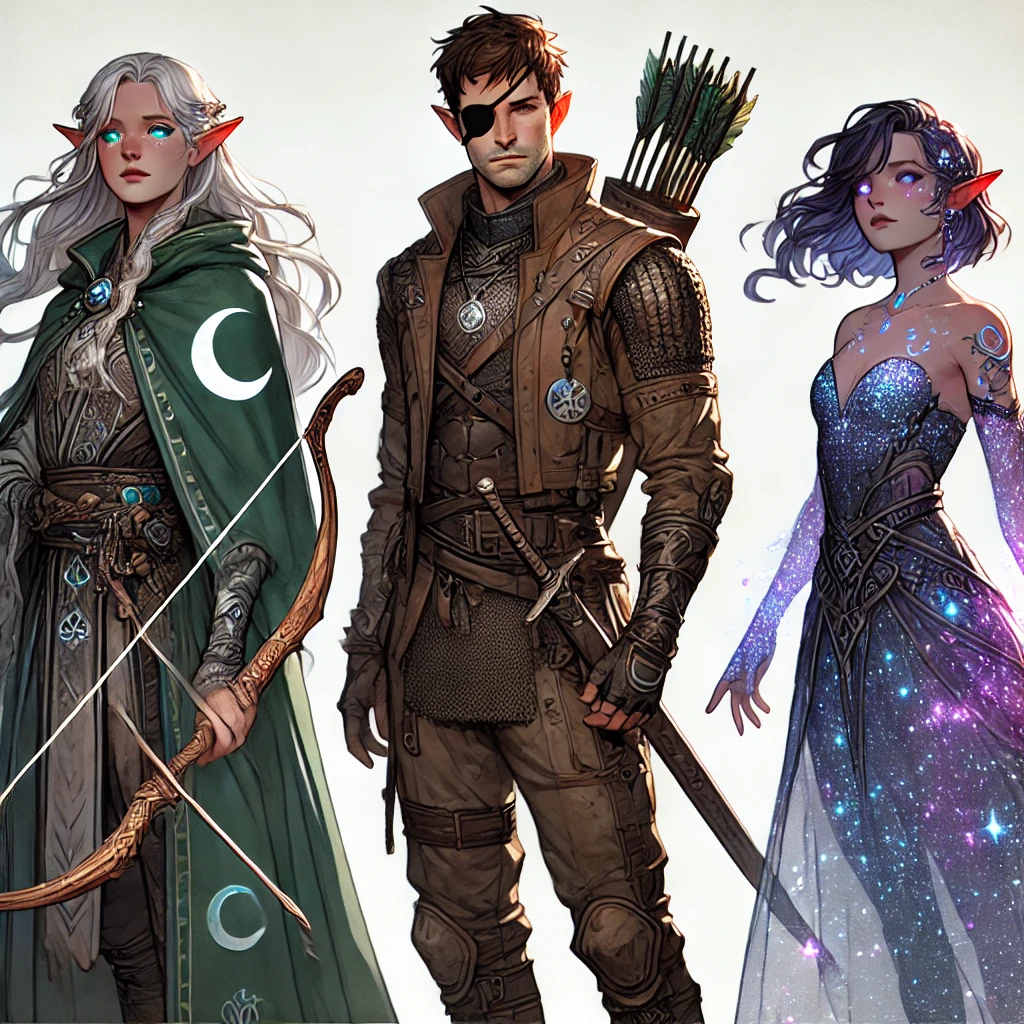
\includegraphics[width=\linewidth]{resources/characters_old}
            \label{fig:char-old-all}
        \end{minipage}
        \hspace{0.01\textwidth}
        \begin{minipage}[t]{0.3\textwidth}
            \centering
            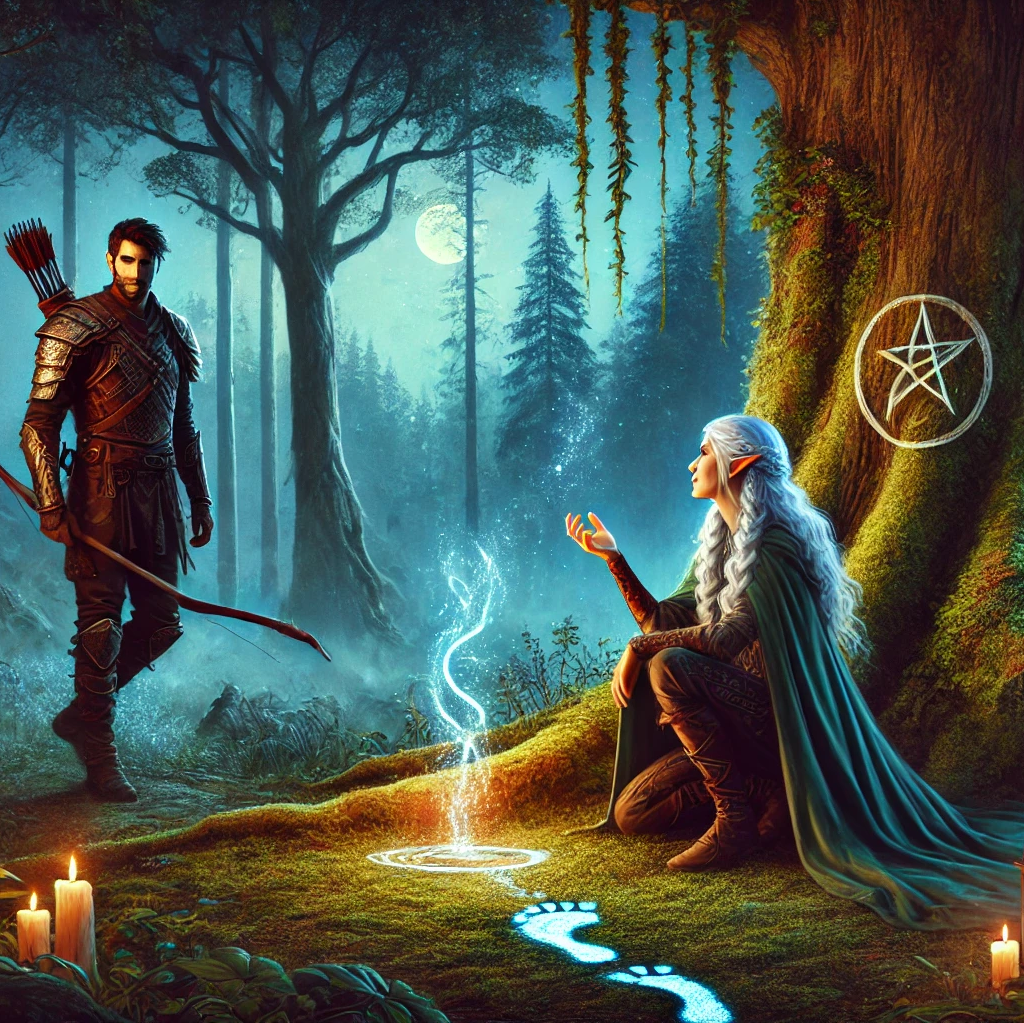
\includegraphics[width=\linewidth]{resources/characters_old_s1}
            \label{fig:char-old-s1}
        \end{minipage}
        \hspace{0.01\textwidth}
        \begin{minipage}[t]{0.3\textwidth}
            \centering
            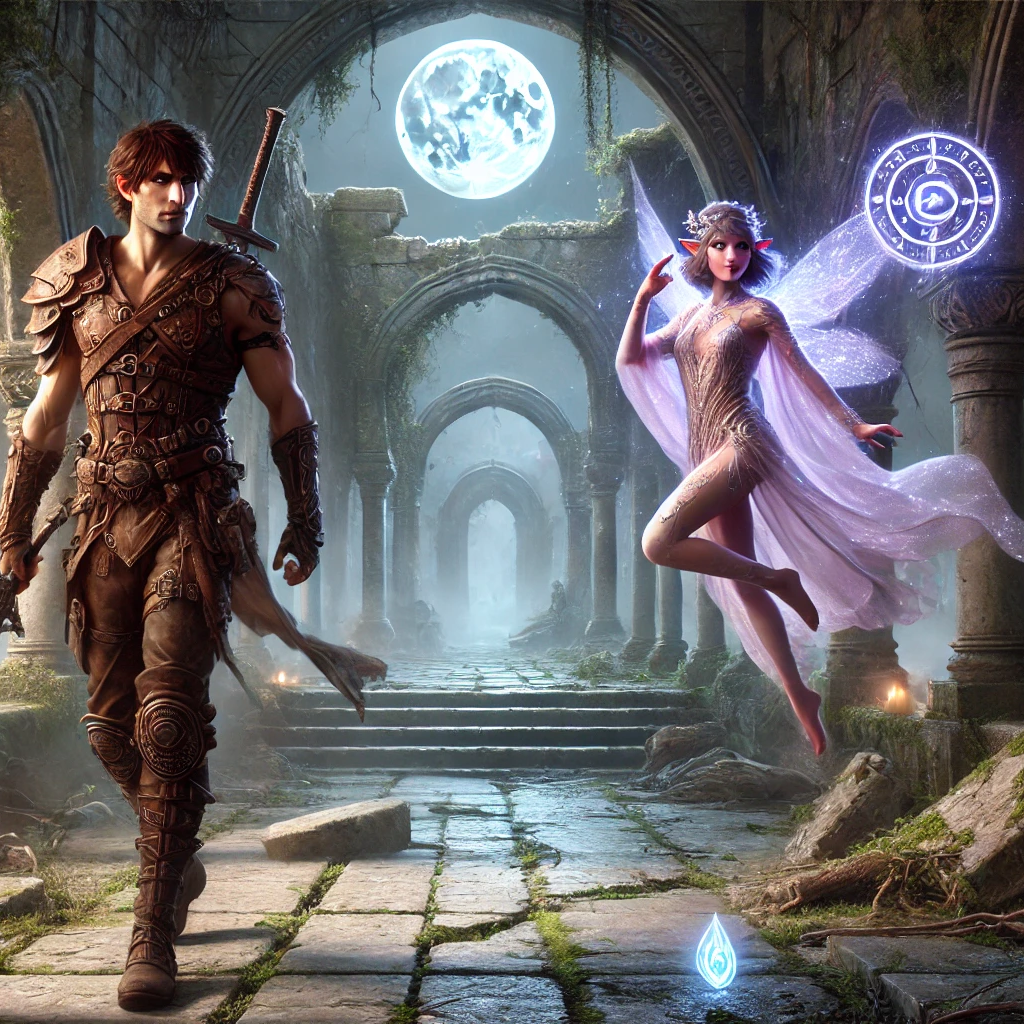
\includegraphics[width=\linewidth]{resources/characters_old_s2}
            \label{fig:char-old-s2}
        \end{minipage}
        \caption{Old model (diffusion-based): Low character consistency.}
        \label{fig:char-old-row}
    \end{subfigure}

    \vspace{1em}

    % ---------------- Row 2: New Model ----------------
    \begin{subfigure}[t]{\textwidth}
        \centering
        \begin{minipage}[t]{0.3\textwidth}
            \centering
            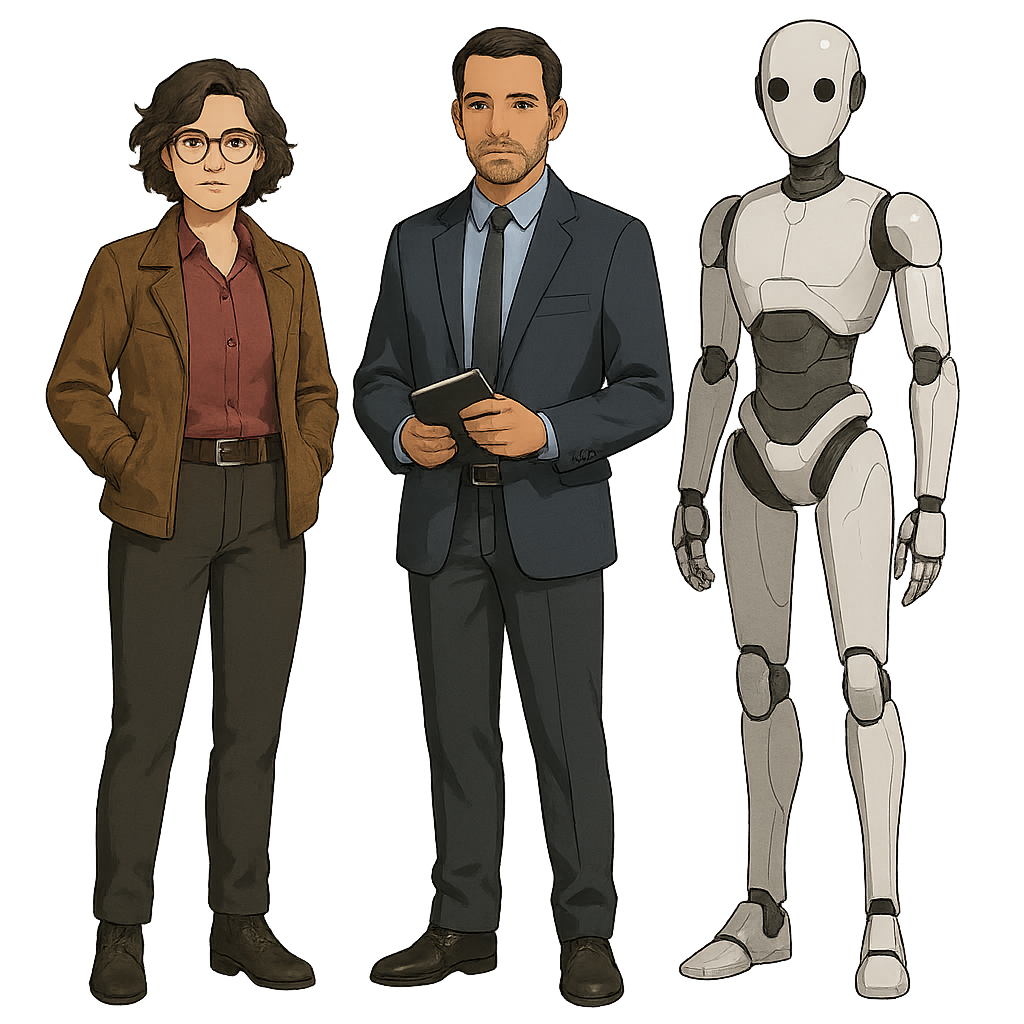
\includegraphics[width=\linewidth]{resources/characters}
            \label{fig:char-new-all}
        \end{minipage}
        \hspace{0.01\textwidth}
        \begin{minipage}[t]{0.3\textwidth}
            \centering
            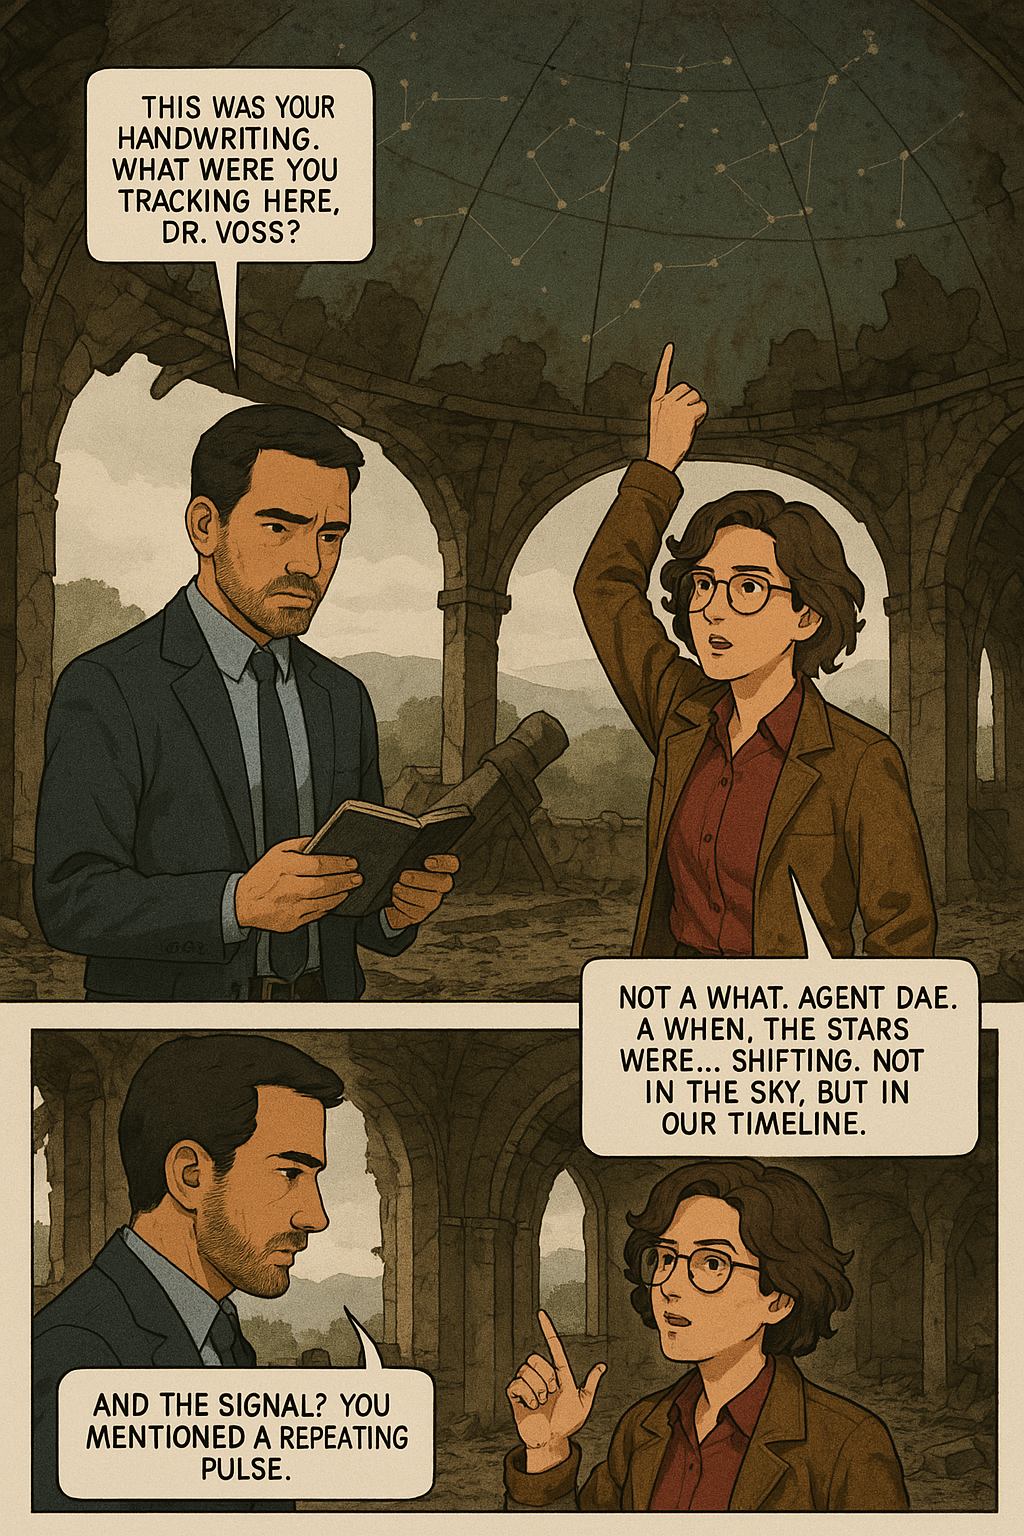
\includegraphics[width=\linewidth]{resources/characters_s1}
            \label{fig:char-new-s1}
        \end{minipage}
        \hspace{0.01\textwidth}
        \begin{minipage}[t]{0.3\textwidth}
            \centering
            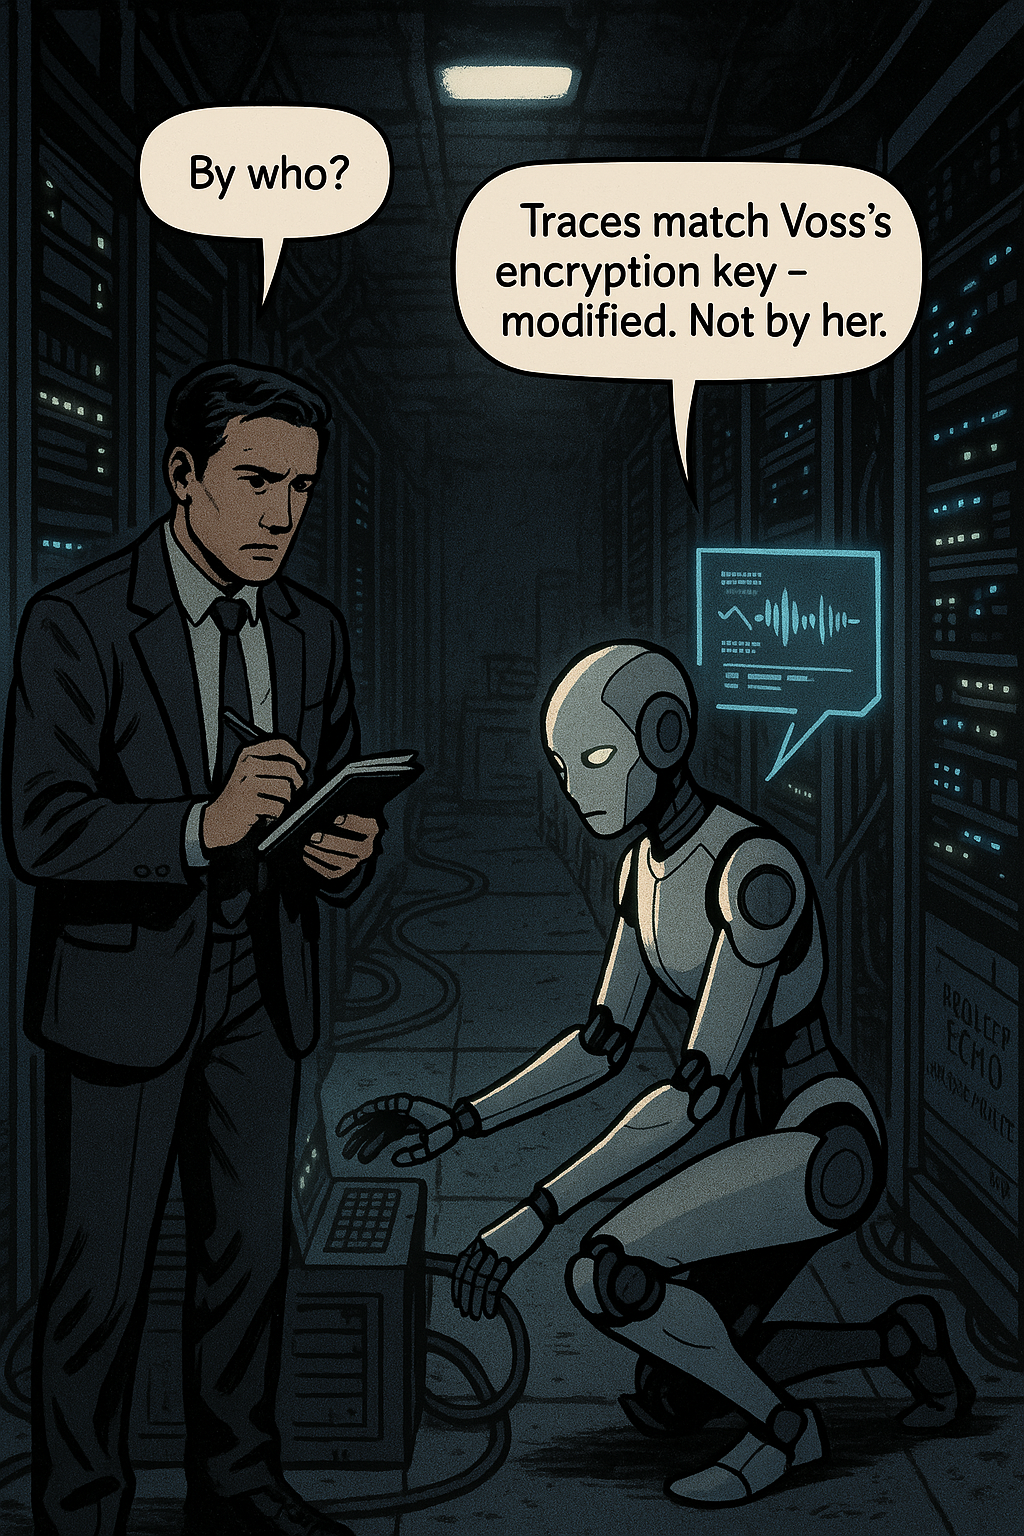
\includegraphics[width=\linewidth]{resources/characters_s2}
            \label{fig:char-new-s2}
        \end{minipage}
        \caption{New model (autoregressive): Character consistency is preserved more effectively.}
        \label{fig:char-new-row}
    \end{subfigure}

    \caption{Comparison of character consistency between the old diffusion-based model and the newer autoregressive model. Each row shows a group portrait and two interaction scenes. The interaction images were truncated to enforce a 1:1 aspect ratio while keeping the key character regions.}
    \label{fig:character-consistency-comparison}
\end{figure*}

\subsection{Multimodal Understanding}\label{subsec:multimodal-understanding}

\textbf{Large Language Models (LLMs)}: An LLM is an autoregressive probabilistic model that predicts
the most probable next token conditioned on user input and previously generated tokens, defined as:
\begin{equation}
    p(w) = \prod_{i=1}^{n} p_{\theta}(w_i \mid w_{<i}),
    \label{eq:llm-autoregressive}
\end{equation}
where $\theta$ represents the parameters of the LLM, typically consisting of multiple layers of transformers.

\textbf{Image LLMs}: Image LLMs equip traditional LLMs with the ability to interpret and understand images.
Their architectures can be categorized into two types: alignment and early fusion~\cite{chen2024multi}.
In the alignment architecture, the image is treated as additional input.
A vision encoder extracts image information, and a trainable alignment module fuses the extracted features
with lexical tokens before passing them through the underlying LLM. Conversely,
the early-fusion architecture trains a multimodal LLM from scratch, directly converting both text and images into tokens.

\subsection{Multimodal Generation}\label{subsec:multimodal-generation}

\textbf{Diffusion Probabilistic Modeling (DDPM)}: DDPM involves a forward and a backward process.
The forward process iteratively adds random Gaussian noise to an input image $x_0$ following a Markov process.
Given a timestep $t$, this process can be represented as:
\begin{equation}
    q(x_t \mid x_{t-1}) = \mathcal{N}(x_t \mid \sqrt{1 - \beta_t} x_{t-1}, \beta_t I),
    \label{eq:forward-ddpm}
\end{equation}
where $\beta_t \in (0,1)$ follows a predefined schedule usually with $\beta_1 < \beta_2 < \dots < \beta_T$.
Typically, $T$ is large enough that $x_T$ approximates pure Gaussian noise.
To generate an image from random noise, the diffusion process is reversed iteratively using a neural network:
\begin{equation}
    p_\theta(x_{t-1} \mid x_t) = \mathcal{N}(x_{t-1} \mid \mu_\theta(x_t, t), \beta_t I),
    \label{eq:reverse-ddpm}
\end{equation}
where $\mu_\theta$ is a neural network parameterized by $\theta$ that predicts
the denoised image $x_{t-1}$ from $x_t$ at timestep $t$.
During training, the objective function is generally defined as:
\begin{equation}
    \min_\theta \mathbb{E}_{x_0, \epsilon, t}[w_t \|\epsilon - \epsilon_\theta(x_t, t)\|_2^2],
    \label{eq:ddpm-loss}
\end{equation}
where $\epsilon$ is randomly sampled noise and $\epsilon_\theta$ is the neural network prediction.

\textbf{Latent Diffusion Models (LDM)}: Diffusion models often expend excessive computational resources
on imperceptible image details.
LDM~\cite{rombach2022high} reduces resource consumption by training diffusion models
on a lower-dimensional latent space $z = E(x)$ compressed via a pretrained autoencoder.
The objective function becomes:
\begin{equation}
    \min_\theta \mathbb{E}_{z_0 = E(x_0), \epsilon, t}[w_t \|\epsilon - \epsilon_\theta(z_t, t, c)\|_2^2],
    \label{eq:ldm-loss}
\end{equation}
where $c$ is an additional condition such as text prompts in text-to-image tasks.

\subsection{Joint Multimodal Understanding and Generation}\label{subsec:joint-multimodal}

\textbf{Joint Autoregressive and Diffusion Models}: Given the strengths of LLMs in text generation and DMs in image generation,
a natural approach to joint multimodal understanding and generation is to integrate an LLM and a DM\@.
Typically, two architectures are possible~\cite{chen2024multi}.
The first involves connecting a pretrained Image LLM and DM, either directly --- though this often struggles
with multimodal generation conditions --- or through training a dedicated connector module.
Nonetheless, this approach is limited by independent modeling.
An alternative is to employ a unified multimodal transformer architecture trained with
both diffusion and autoregressive regularization.
In Transfusion~\cite{zhou2024transfusion}, texts are processed through embedding matrices,
and local $k\times k$ image patches are compressed into single transformer vectors via neural networks employing
hybrid attention mechanisms (causal and bidirectional).
During denoising, pure noise in the form of $n$ image patches is appended to the input sequence
and iteratively denoised over $T$ steps by the transformer.

\textbf{Autoregressive Image Generation}: Previous approaches, such as Chameleon~\cite{team2024chameleon},
tokenize images into discrete tokens using a codebook, mixing them with text tokens in
a unified multimodal autoregressive model to generate mixed outputs.
Despite these efforts, this method still encounters two key issues~\cite{chen2024multi},
1) the tokenizer's codebook derived from an image reconstruction objective predominantly captures pixel-level
rather than semantic information;
and 2) discretization inevitably results in visual information loss,
negatively affecting tasks requiring fine-grained image understanding.

\textbf{Autoregressive Generation without Vector Quantization}: MAR~\cite{li2024autoregressive} proposes generating images
with masked autoregressive modeling without quantizing image tokens.
This approach models per-token distributions using a diffusion process on continuous-valued domains.
Traditionally, generated continuous-valued vectors $z$ are projected onto a discrete domain through a classifier matrix $W$:
\begin{equation}
    p(x \mid z) = \text{softmax}(W z).
    \label{eq:softmax-projection}
\end{equation}
Alternatively, MAR formulates this probability as a diffusion-based denoising criterion:
\begin{equation}
    \mathcal{L}(z, x) = \mathbb{E}_{\epsilon, t}[\|\epsilon - \epsilon_\theta(x_t, t, z)\|_2^2].
    \label{eq:mar-loss}
\end{equation}

\subsection{Challenges in Comic Generation}\label{subsec:challenges-in-comic-generation}

Despite advancements in controllable diffusion-based generation methods like Textual Inversion~\cite{gal2022image}
and Dreambooth~\cite{ruiz2023dreambooth}, commercially available image generation systems rarely allow end-users
to customize models at training time.
This significantly hinders consistently representing specific artistic styles across different scenes.
Additionally, traditional diffusion-based methods have limited accuracy in rendering text within images.
Notably, OpenAI's recently announced ChatGPT-4o (March 25, 2025)~\cite{openai2025introducing} is
a unified multimodal autoregressive model that generates clear text and consistent characters
without additional training --- an essential requirement for comic creation.
